\documentclass{amsart}
\usepackage[utf8]{inputenc}
\usepackage{graphicx}

\title{Fritter Design \\ For a more potato-ey tomorrow}
\author{Evan Lynch}
\date{October 1, 2014}

\begin{document}
\maketitle
\section{Terminology}
Since this is \emph{Fritter} and not \emph{Twitter}, the \emph{Tweet} analog is
called a  \emph{Frite}. To deliver a \emph{Frite},
one must \emph{Fry} it, making the deliverer a \emph{Fryer}. Additionally, since one often
pays for a potato with dollars and cents, to tag a \emph{Frite} one would use a 
``\$cashtag.'' If one found a \emph{Frite} to their liking and wanted to \emph{Fry} it
themselves without modification, this would be called \emph{refry}-ing.

\section{Highlights}
\label{sec:subtitle}
The potato spinner GIF that shows up when the UI is blocking is the clear winner. However, another
highlight is the simple API. The API is good because it is fully specified in terms of inputs, outputs, and side-effects, and though limited in scope, it is designed without a particular client in mind. This made
writing the REACT client-side app much easier.

The ``features'' I chose to implement beyond the basic requirements of a Twitter-like app are:
\begin{enumerate}
\item Following -- the user may add other users to their following list; then they can see only what their friends are frying in a special aggregated view.
\item Refrying -- the user may, with a single click, quote and share the frite of another user.
\item Search - the user may choose to see only frites that include selected \$cashtags or only frites from selected other users denoted in the search bar as @username. Message body search is not implemented.
\end{enumerate}

\section{Design Challenges}
\label{sec:another_subtitle}
The main design decisions to make were the following.
\begin{enumerate}
\item What schema and structure to select for the data model
\item How much view rendering to do client-side / what view end-points to support
\item What interface to expose through an API to the client
\item How to model data on the client side
\item How to render views on the client side
\end{enumerate}
Now, I will describe the decision I made for each and why.

\subsection{Data Model}
\begin{figure}[htbp]
    \centering
    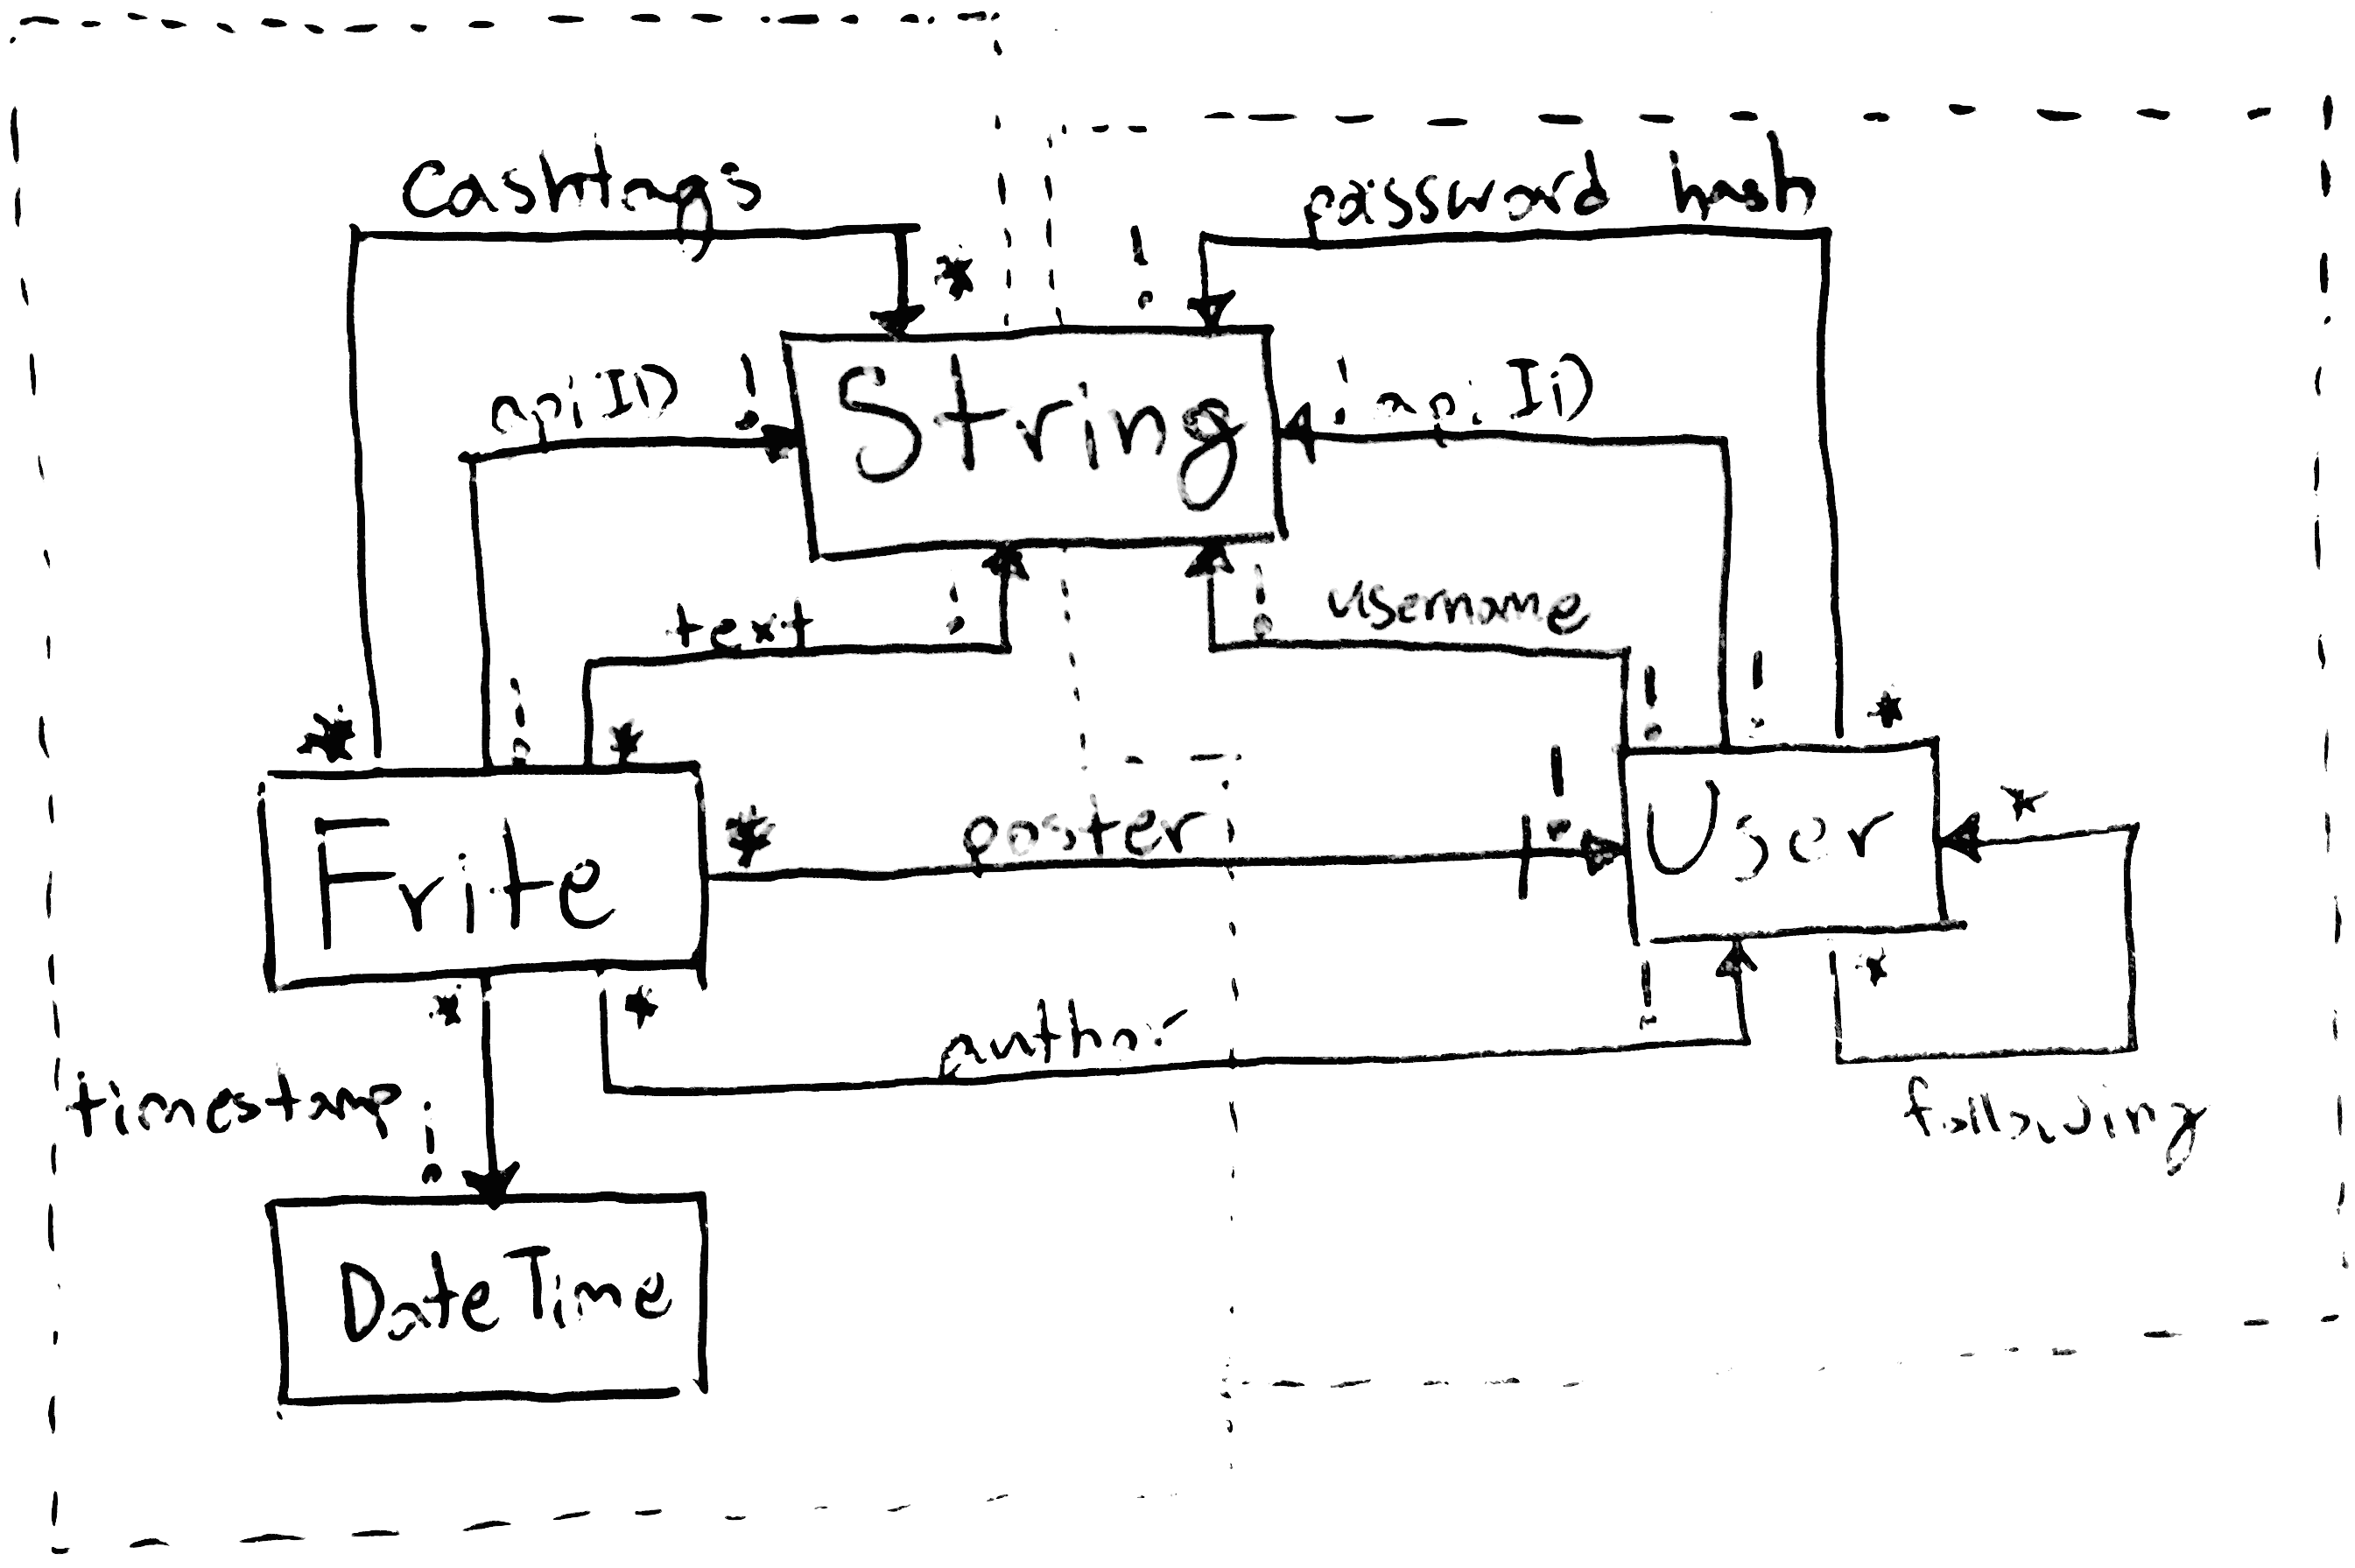
\includegraphics[width=0.95\textwidth]{model.png}
    \caption{Data Model}
    \label{fig:datamodel}
\end{figure}
The data model is presented in Figure~\ref{fig:datamodel}. I chose to use the mongoose wrapper for MongoDB.
Out of the data model come two obvious structures which have been represented with the following schema
defined in model.js
\begin{verbatim}
User:
    username: String
    hash: String
    apiID: String of the form u_??????????
    following: Array of (ObjectID referencsing users collection)

Frite:
    text: String
    timestamp: Date (serialized by mongoose)
    apiID: String of the form fr_??????????
    cashtags: Array of Strings
    poster: Number (ObjectID referencing users collection)
    author: Number (ObjectID referencing users collection)
\end{verbatim}
The data model was chosen to facilitate the functions of the application. First, each Frite
carries a reference to a User document rather than a nested user to avoid excesive repetition
and to make it easier to make modifications the the user part of the data model.

Second, both an ``author'' and a ``poster'' reference are stored for by the each Frite
to facilitate the `refry' feature. When a Frite is refried the author of the new Frite
is set to the original Frite's author. If it is later edited, the new Frite's author is
changed to the poster.

Third, the User carries an array of references to other users implementing a list to be followed.
This relation was chosen (rather than the reverse), because the primary function of following
is to allow the user to quickly see the posts of the users they are following (rather than
to see who is following them, although this could be desired as well).

Finally, the data model was selected so that only one level of mongoose.populate would be required
for the functionality of the application.

\subsection{Views}
I opted to do the vast majority of view rendering on the client side. The server only
responds with HTML at two end-points ``/'' and ``/login'' routed in views.js.
The ``/login'' end-point
allows a user to log in regardless of what username is set in the session while the
``/'' end-point goes to the main site unless there is no username set in the session
in which case it goes to the login page. The HTML response on both of these do little
more than load the client-side javascript and set globally scoped variable ``bootstrap''
in which it passes the username from the session. For the small amount of templating
this required, I used the Jade template engine.


\subsection{API}
The API was designed as a ``public'' API taking the perspective that any API that the
server presents as an interface is ``public'' to begin with in the sense that anyone
can send it requests not just the designated client app. Therefore, it sends and
receives JSON and attempts to return helpful error messages and status codes when
requests are formatted wrong or fail for other reasons. The interface is well documented
in api.js.


\subsection{Client-side}
I chose to use Backbone.js for storing a model of responses from the API in the client app. I use
little of Backbone's functionality otherwise, but the Backbone model was a convenient choice for
parsing performing API fetches and saving them in a coherent manner and keeping them in sorted order.

The client implements the view with REACT.js which is a framework for writing reactive client-side
applications in a declarative fashion. The structure of a view in REACT is a hierarchy of components
each which can carry and update state as well as pass down properties to children. The UI is declared
to appear a certain way based on the state and properties that the component has. My REACT code has
the following structure.
\begin{figure}[htbp]
    \centering
    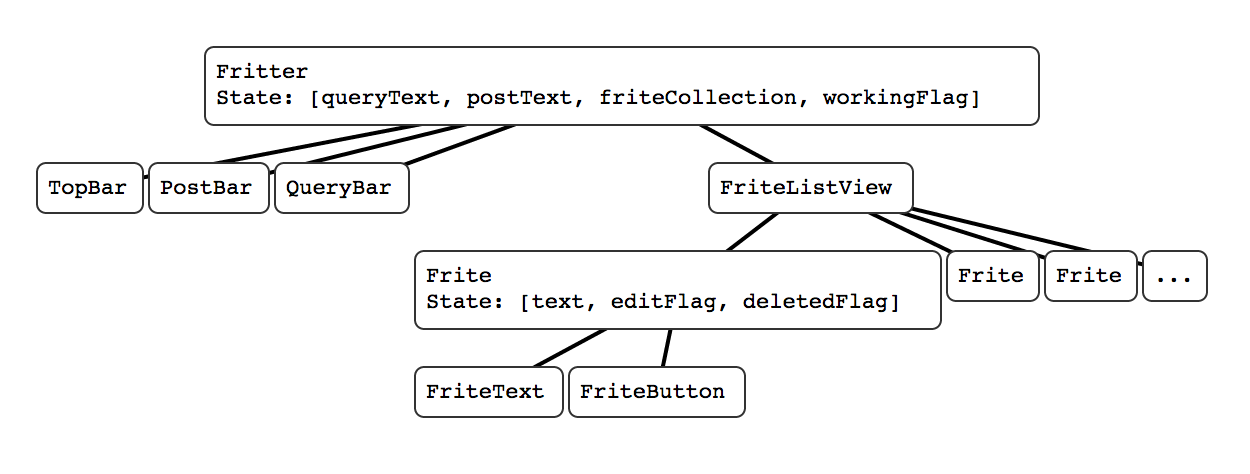
\includegraphics[width=0.95\textwidth]{reacttree}
\end{figure}


\end{document}